\documentclass{article}
\usepackage{tikz}
\usetikzlibrary{matrix, arrows}

\begin{document}

\begin{figure}[h]
    \centering
    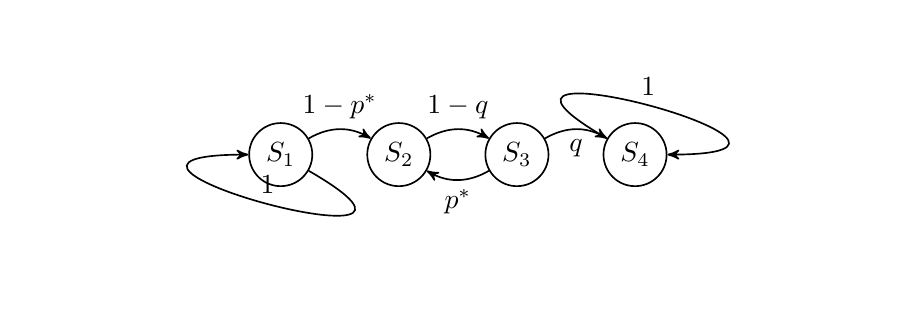
\begin{tikzpicture}[->, >=stealth', semithick, auto, node distance=1.5cm, main/.style = {draw, circle}]
        \node[main] (s1) {$S_{1}$};
        \node[main] (s2) [right of=s1] {$S_{2}$};
        \node[main] (s3) [right of=s2] {$S_{3}$};
        \node[main] (s4) [right of=s3] {$S_{4}$};

        \path (s1) edge[out=-30,in=180,looseness=9, above] node[above] {$1$} (s1);
        \path (s1) edge[bend left] node[above] {$1 - p^{*}$} (s2);
        \path (s2) edge[bend left] node[above] {$1 - q$} (s3);
        \path (s3) edge[bend left] node[below] {$p^{*}$} (s2);
        \path (s3) edge[bend left] node[below] {$q$} (s4);
        \path (s4) edge[out=150,in=0, looseness=9, above] node[above] {$1$} (s4);
    \end{tikzpicture}
    \caption{The Markov chain for the process of Lemma \ref{lem:lower_mutant}. $S_2 = \Config$, $S_3 = \Config^\star$, $S_4 = \Config^+$}
    \label{fig:markov_chain}
\end{figure}

\end{document}